\subsection{Characteristic as function of light intensity}
\begin{table}[H]
    \centering
    \begin{tabular}{@{}cc@{}}
\toprule
\textbf{Variac (Volts)} & \textbf{Light Intensity(Amps)}  \\ \midrule
        120             &         446                       \\        
        110             &        363                        \\         
        100             &       285                         \\    
        90              &        220                        \\     
        80              &       159                         \\  
        70              &        109                        \\ 
        60              &        68                       \\
        50              &        37                        \\
        40              &       16                          \\
        30              &        6.4                         \\
        20              &       1.7                         \\
        10              &         1.0                      \\ \bottomrule
\end{tabular}
    \caption{Variac versus Light Intensity}
    \label{tab:variac_data}
\end{table}

\begin{table}[H]
    \centering
    \begin{tabular}{@{}ccccc@{}}
\toprule
\multicolumn{1}{c}{\multirow{2}{*}{\textbf{\begin{tabular}[c]{@{}c@{}}Variac\\ (Volts)\end{tabular}}}} & \multicolumn{2}{c}{\textbf{$V_{oc}$}}                                                           & \multicolumn{2}{c}{\textbf{$I_{sc}$}}                                                           \\ \cmidrule(lr){2-3} \cmidrule(lr){4-5} 
\multicolumn{1}{c}{}                                                                                   & \multicolumn{1}{c}{\textbf{$V_{oc}$ (V)}} & \multicolumn{1}{c}{\textbf{Thermistor ($K\Omega$)}} & \multicolumn{1}{c}{\textbf{$I_{sc}$ (A)}} & \multicolumn{1}{c}{\textbf{Thermistor ($K\Omega$)}} \\ \midrule
%V      V_oc        thermo      I_sc        thermo
120 &    2.42       & 5.12  &    0.00594       & 5.11           \\
110 &   2.38        & 5.13  &    0.00449       & 5.12           \\
100 &   2.34        & 5.11  &    0.00335       & 5.11          \\
90  &   2.30        & 5.10  &    0.00229       & 5.10          \\
80  &   2.24        & 5.10  &    0.00154       & 5.09          \\
70  &   2.18        & 5.09  &    0.00093       & 5.08          \\
60  &   2.11        & 5.10  &    0.00056       & 5.09          \\
50  &   2.04        & 5.10  &    0.00036       & 5.08          \\
40  &  1.98         & 5.10  &    0.00026       & 5.087          \\
30  &  1.95         & 5.108 &    0.00021       & 5.090          \\
20  &  1.942        &5.120  &    0.00021       & 5.094          \\
10  &  1.946        &5.126  &    0.00021       & 5.098          \\
 \bottomrule
\end{tabular}
    \caption{Open Circuit Voltage and Short Circuit Current}
    \label{tab:open_closed_data}
\end{table}

\subsection{Temperature Dependence of no-load voltage}

\begin{table}[H]
    \centering
    \begin{tabular}{@{}ccc@{}}
\toprule
\multicolumn{1}{c}{\textbf{\begin{tabular}[c]{@{}c@{}}Thermistor around 5k \\ $\sim$23$^\circ$C (Room Temp)\end{tabular}}} & \textbf{Fluke IR ($^\circ$C)} & \multicolumn{1}{c}{\textbf{\begin{tabular}[c]{@{}c@{}}V$_{oc}$ at 60V \\ Vairac\end{tabular}}} \\ \midrule
% resist || TEMP     || Voltage OC
 5.149       & room temp(24.0)        &  1.9206     \\
 4.28        &   30.0        &  1.886      \\
4.99        &   35.0         &  1.918     \\
3.51        &   40.0         &  1.872      \\
3.13        &   45.0         &  1.839      \\
2.45        &   50.0         &  1.841     \\
1.81        &   55.0         &  1.780      \\
1.76        &   61.2         &  1.752      \\
1.72        &   65.0         &  1.710      \\
1.38        &   69.6         &  1.688      \\
1.18        &   75.1         &  1.631     \\
 0.96       &  80 $^\circ$C (max) &      1.571\\ \bottomrule
\end{tabular}
    \caption{Temperature Effect on $V_{oc}$}
    \label{tab:temp_effect_data}
\end{table}
\clearpage
\subsection{I-V characteristics of the solar cell}

\begin{figure}[ht] 
  \begin{subfigure}[b]{0.5\linewidth}
    \centering
    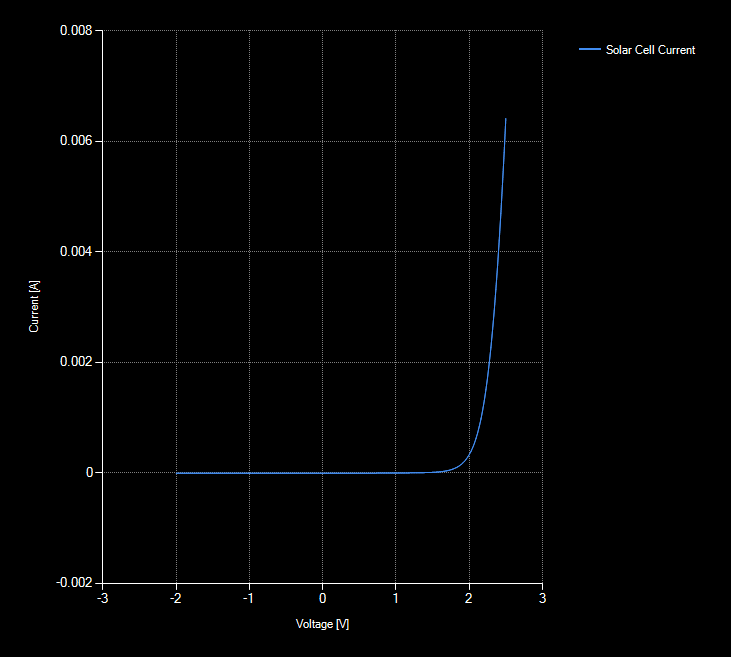
\includegraphics[width=0.90\linewidth]{figures/DarkChar.png} 
    \caption{Dark enclosure} 
    \label{fig:dark} 
    \vspace{4ex}
  \end{subfigure}%% 
  \begin{subfigure}[b]{0.5\linewidth}
    \centering
    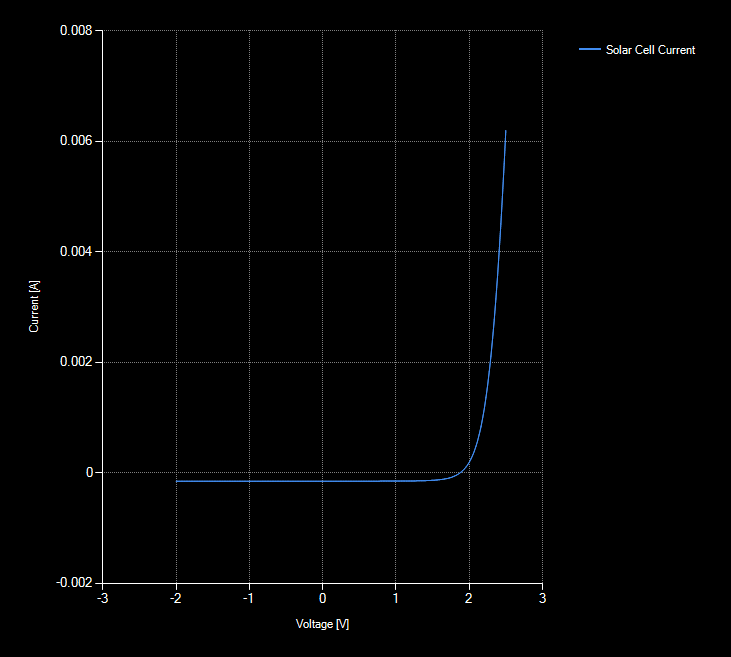
\includegraphics[width=0.90\linewidth]{figures/30VChar.png} 
    \caption{Light at variac = 30V } 
    \label{fig:30} 
    \vspace{4ex}
  \end{subfigure} 
  \begin{subfigure}[b]{0.5\linewidth}
    \centering
    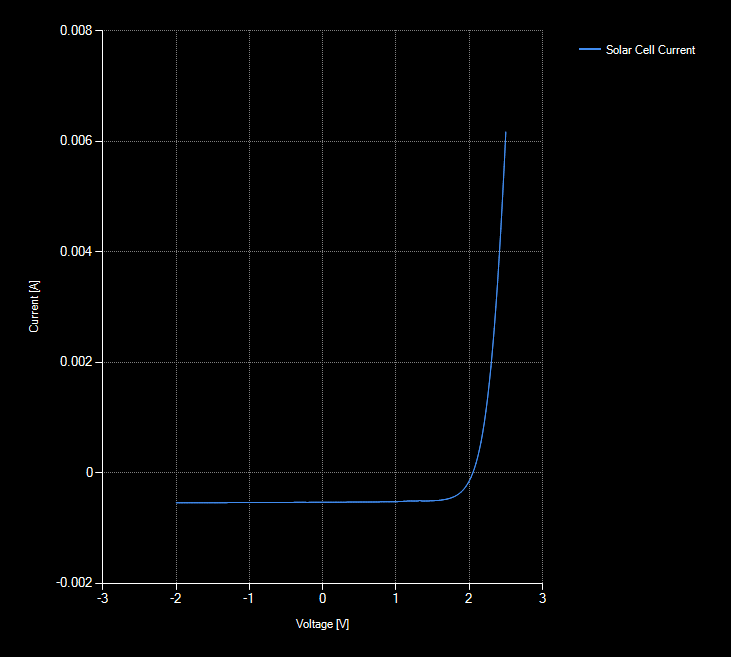
\includegraphics[width=0.90\linewidth]{figures/60VChar.png} 
    \caption{Light at variac = 60V} 
    \label{fig:60} 
  \end{subfigure}%%
  \begin{subfigure}[b]{0.5\linewidth}
    \centering
    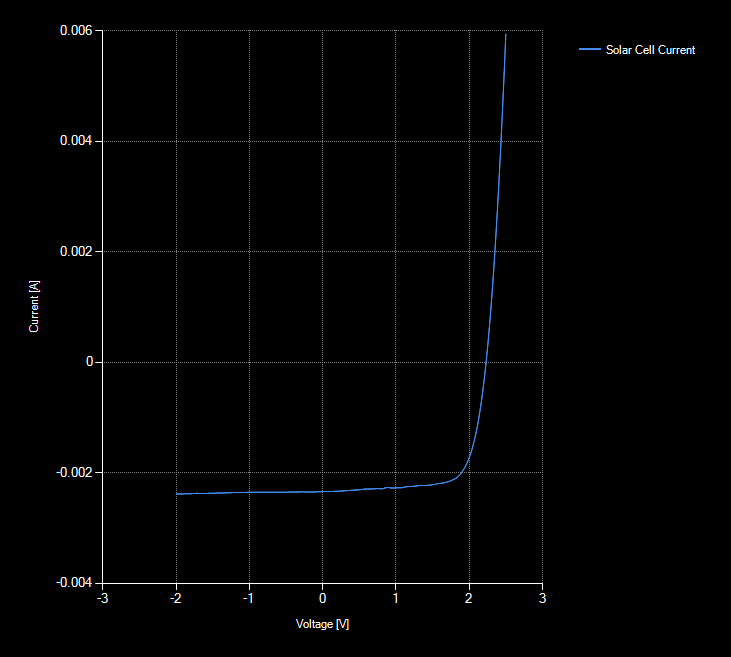
\includegraphics[width=0.90\linewidth]{figures/90VChar.png} 
    \caption{Light at variac = 90V} 
    \label{fig:90} 
  \end{subfigure} 
  \caption{Solar cell I-V characteristics captured in various lighting conditions}
  \label{fig:IV} 
\end{figure}

\clearpage

\subsection{Carrier life time, response time }

\begin{figure}[h]
    \centering
    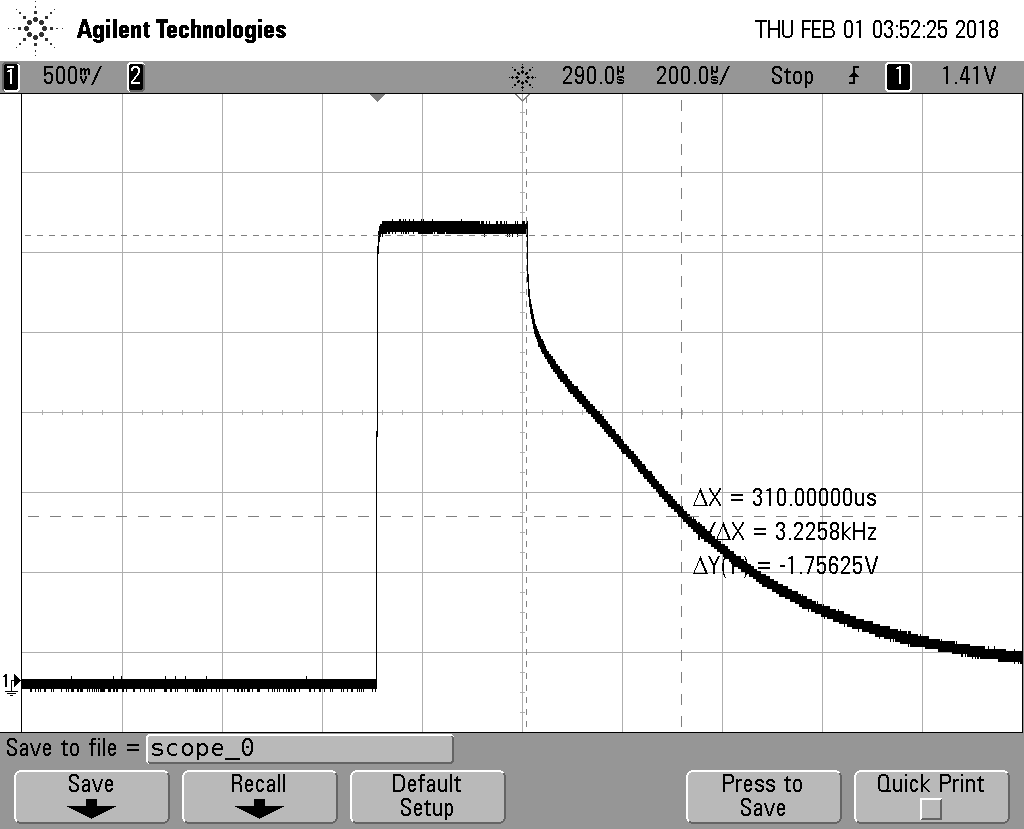
\includegraphics[width=.75\linewidth]{figures/carrier.png}
    \caption{Carrier decay time, decay time indicators measured from 100\% to 37\%}
    \label{fig:carrier}
\end{figure}